\chapter{Конструкторская часть}
В данном разделе будут реализованы схемы алгоритмов умножения матриц и будут приведены рассчеты трудоемкостей для этих алгоритмов.

\section{Разработка алгоритмов}
На рисунке \ref{fig:Stand} представлена схема алгоритма для стандартного умножения.

На рисунках \ref{fig:Vinograd1}--\ref{fig:Vinograd2} представлены схемы алгоритма умножения методом Винограда.

На рисунках \ref{fig:VinogradOpt1}--\ref{fig:VinogradOpt2} представлены схемы оптимизированного алгоритма умножения методом Винограда.

\begin{figure}[h]
	\centering
	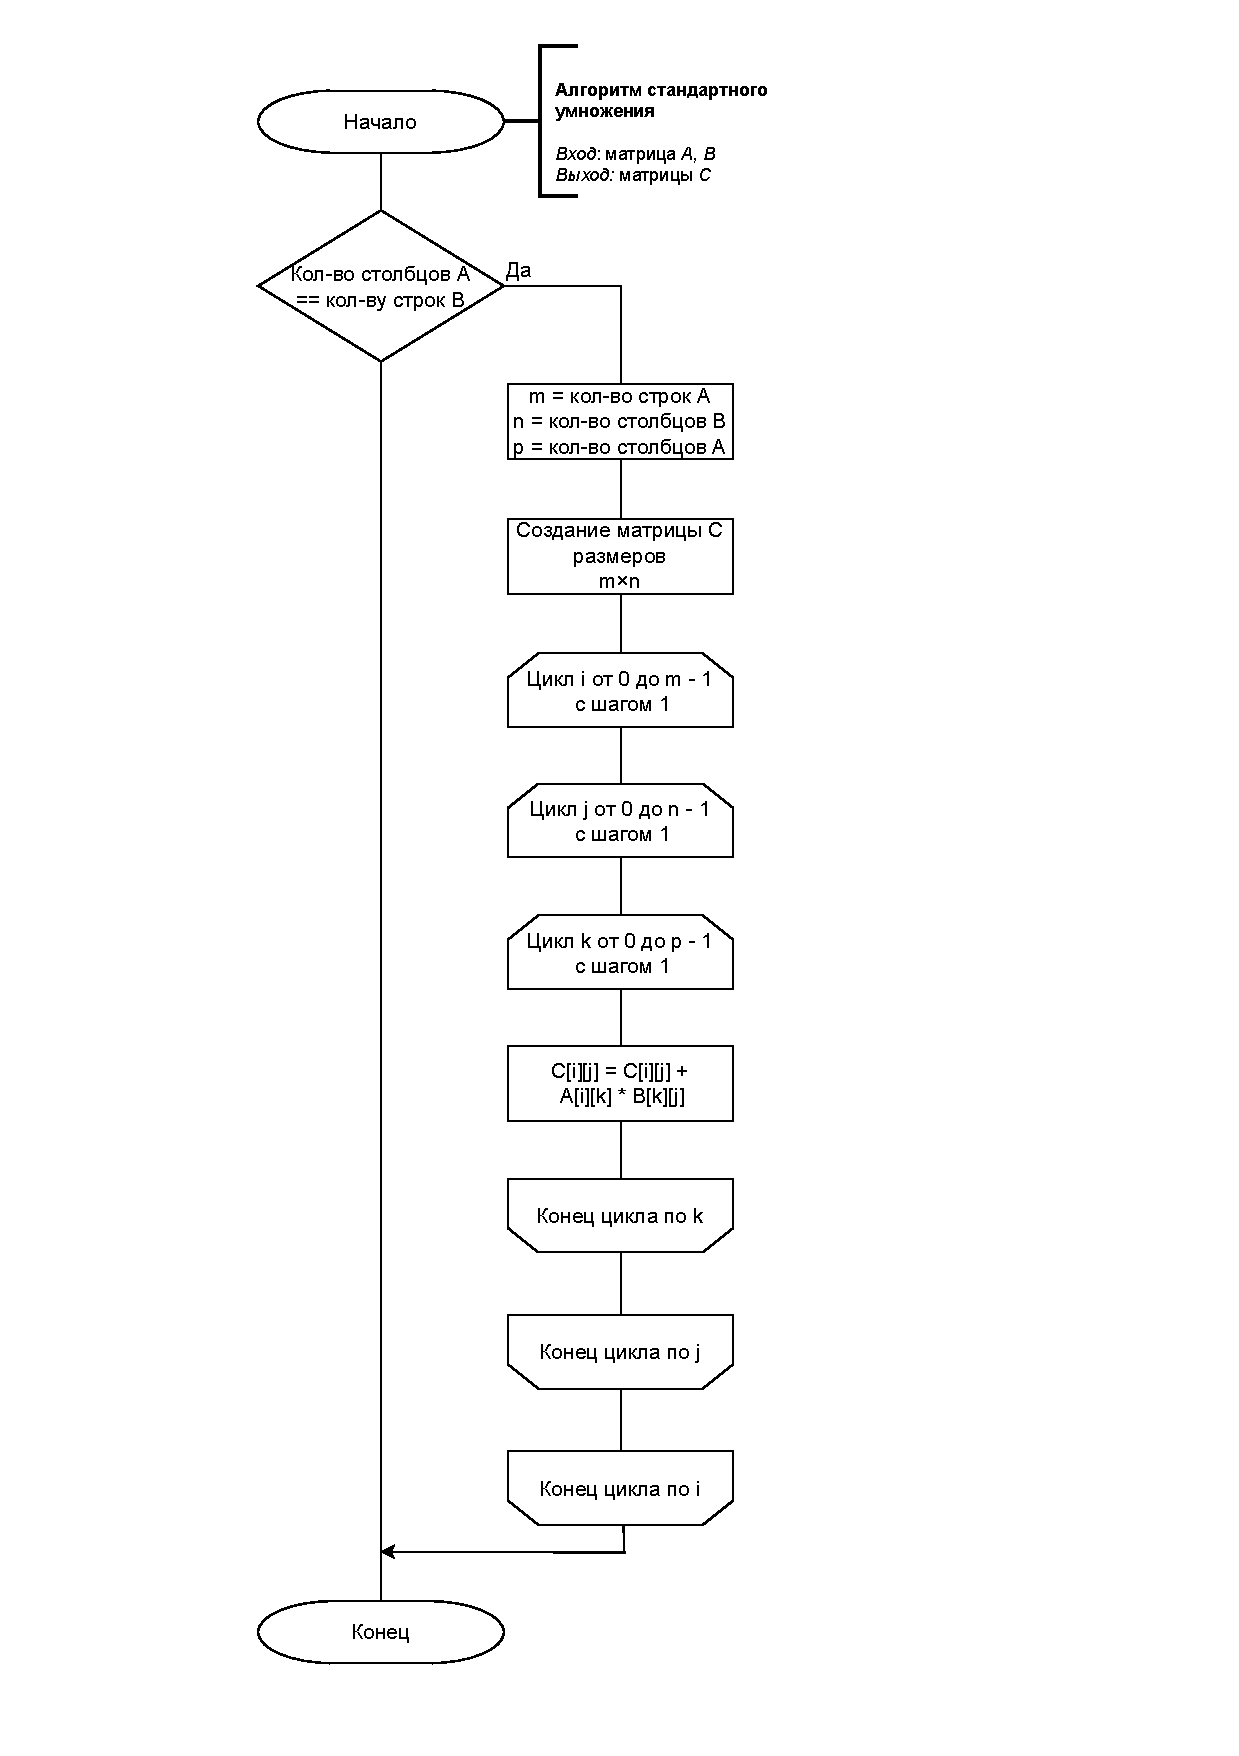
\includegraphics[height=0.9\textheight, page=1]{img/algorithms.pdf}
	\caption{Схема стандартного алгоритма умножения матриц}
	\label{fig:Stand}
\end{figure}

\clearpage

\begin{figure}[h]
	\centering
	\includegraphics[height=0.9\textheight, page=2]{img/algorithms.pdf}
	\caption{Схема алгоритма умножения матриц методом Винограда (начало)}
	\label{fig:Vinograd1}
\end{figure}

\clearpage

\begin{figure}[h]
	\centering
	\includegraphics[height=0.9\textheight, page=3]{img/algorithms.pdf}
	\caption{Схема алгоритма умножения матриц методом Винограда (конец)}
	\label{fig:Vinograd2}
\end{figure}

\clearpage

\begin{figure}[h]
	\centering
	\includegraphics[height=0.9\textheight, page=4]{img/algorithms.pdf}
	\caption{Схема оптимизированного алгоритма умножения матриц методом Винограда (начало)}
	\label{fig:VinogradOpt1}
\end{figure}

\clearpage

\begin{figure}[h]
	\centering
	\includegraphics[height=0.9\textheight, page=5]{img/algorithms.pdf}
	\caption{Схема оптимизированного алгоритма умножения матриц методом Винограда (конец)}
	\label{fig:VinogradOpt2}
\end{figure}

\clearpage

\section{Модель вычислений для проведения оценки трудоемкости алгоритмов}
Для последующего вычисления трудоемкости необходимо ввести модель вычислений:

\begin{enumerate}
	\item операции из списка \ref{eq:operations1} имеют трудоемкость \textbf{1};
	\begin{equation}
		\label{eq:operations1}
		\begin{gathered}
			+, -, =, +=, -=, ==, !=, <, >, <=, >=, [], \\ ++, --, \&\&, >>, <<, ||, \&, |
		\end{gathered}
	\end{equation}
	\item операции из списка \ref{eq:operations2} имеют трудоемкость \textbf{2};
	\begin{equation}
		\label{eq:operations2}
		*, /, \%, *=, /=, \%=
	\end{equation}
	\item трудоемкость условного оператора \texttt{if условие then A else B} рассчитывается как \ref{eq:if};
	\begin{equation}
		\label{eq:if}
		f_{if} = f_{\text{условия}} + 
		\begin{cases}
			f_{A}, & \text{в случае выполнеия условия,}\\
			f_{B}, & \text{иначе}.
		\end{cases}
	\end{equation}
	\item трудоемкость цикла рассчитывается как \ref{eq:for}
	\begin{equation}
		\label{eq:for}
		\begin{gathered}
			f_{for} = f_{\text{инициализация}} + f_{\text{сравнения}} + M_{\text{итераций}} \cdot (f_{\text{тело}} +\\
			+ f_{\text{инкремент}} + f_{\text{сравнения}});
		\end{gathered}
	\end{equation}
	\item трудоемкость вызова функции равна 0.
\end{enumerate}

\section{Трудоемкость алгоритмов}
В следующих частях будут приведены рассчеты трудоемкостей алгоритмов для умножения матриц.

Пусть у нас есть 2 матрицы: 
\begin{enumerate}
	\item $A$ размером $M \times P$;
	\item $B$ размером $P \times N$.
\end{enumerate}

\subsection*{Стандартный алгоритм}
Трудоемкость стандартного алгоритма умножения матриц состоит из:
\begin{itemize}
	\item внешнего цикла по $i \in [1 \ldots M]$ , трудоёмкость которого: $f = 2 + M \cdot (2 + f_{body})$;
	\item цикла по $j \in [1 \ldots N]$ , трудоёмкость которого: $f = 2 + N \cdot (2 + f_{body})$;
	\item цикла по $k \in [1 \ldots P]$ , трудоёмкость которого: $f = 2 + K \cdot (2 + 12)$;
\end{itemize}
Так как трудоемкость стандартного алгоритма равно трудоемкости внешнего цикла~--- можно вычислить ее, подставив циклы тела:
\begin{equation}
	\begin{gathered}
		f_{standart} = 2 + M \cdot (2 + 2 + N \cdot (2 + 2 + P \cdot (2 + 8 + 1 + 1 + 2))) = \\
		= 2 + 4M + 4MN + 14MNP \approx 14MNP = O(N^3).
	\end{gathered}
\end{equation}

\subsection*{Алгоритм Винограда}
При вычислении трудоемкости алгоритма Винограда необходимо учесть следующее:
\begin{itemize}
	\item трудоемкость создания и инициализации массивов \textit{MulH} и \textit{MulV}:
	\begin{equation}
		f_{init} = f_{MulH} + f_{MulV};
	\end{equation}
	\item трудоемкость заполнения массива \textit{MulH}:
	\begin{equation}
		\begin{gathered}
		f_{MulH} = 2 + M \cdot (2 + 4 + \frac{P}{2} \cdot (4 + 6 + 1 + 2 + 3 \cdot 2)) = \\
		= 2 + 6M + \frac{19MP}{2};
		\end{gathered}
	\end{equation}
	\item трудоемкость заполнение массива \textit{MulV}:
	\begin{equation}
		\begin{gathered}
		f_{MulV} = 2 + N \cdot (2 + 4 + \frac{P}{2} \cdot (4 + 6 + 1 + 2 + 3 \cdot 2)) = \\
		= 2 + 6N + \frac{19NP}{2};
		\end{gathered}
	\end{equation}
	\item трудоемкость цикла заполения для четных размеров:
	\begin{equation}
		\begin{gathered}
			f_{cycle} = 2 + M \cdot (4 + N \cdot (13 + \frac{P}{2} \cdot 32)) = 2 + 4M + \\
			+ 13MN + \frac{32MNP}{2}  = 2 + 4M + 13MN + 16MNP;
		\end{gathered}
	\end{equation}
	\item трудоемкость дополнительного цикла, в случае нечетного размера матрицы:
	\begin{equation}
		\begin{gathered}
			f_{check} = 3 + 
			\begin{cases}
				0, & \text{чётная} \\
				2 + M \cdot (4 + N \cdot (2 + 14)), & \text{иначе}.
			\end{cases}
		\end{gathered}  
	\end{equation}
\end{itemize}
В итоге, для худшего случая (т. е. когда размер матрицы нечетный) получаем следующую трудоемкость:
\begin{equation}
	f_{worst} = f_{MulH} + f_{MulV} + f_{cycle} + f_{check} \approx 16MNP = O(N^3).
\end{equation}
Для лучшего случая (т. е. когда размер матрицы четный):
\begin{equation}
	f_{best} = f_{MulH} + f_{MulV} + f_{cycle} + f_{check} \approx 16MNP = O(N^3).
\end{equation}

\subsection*{Оптимизированный алгоритм Винограда}
Оптимизация алгоритма Винограда осуществляется за счет следующего набора действий:
\begin{itemize}
	\item замены операции $x = x + k$ на $x += k$;
	\item замены $\cdot 2$ на $<<$;
	\item предвычисления некоторых слагаемых для алгоритма.
\end{itemize}
Итоговая трудоемкость оптимизированного алгоритма Винограда состоит из:
\begin{itemize}
	\item трудоемкости кеширования значения $\frac{P}{2}$~--- 3;
	\item трудоемкость заполнения массива \textit{MulH}:
	\begin{equation}
		\begin{gathered}
			f_{MulH} = 2 + M \cdot (2 + 2 + \frac{P}{2} \cdot (2 + 5 + 1 + 2 + 3)) = \\
			= 2 + 2M + \frac{13MP}{2};
		\end{gathered}
	\end{equation}
	\item трудоемкость заполнение массива \textit{MulV}:
	\begin{equation}
		\begin{gathered}
			f_{MulV} = 2 + N \cdot (2 + 2 + \frac{P}{2} \cdot (2 + 5 + 1 + 2 + 3)) = \\
			= 2 + 2N + \frac{13NP}{2};
		\end{gathered}
	\end{equation}
	\item трудоемкость цикла заполения для четных размеров:
	\begin{equation}
		\begin{gathered}
			f_{cycle} = 2 + M \cdot (4 + N \cdot (2 + 10 + 2 + \frac{P}{2} \cdot 19)) = \\
			= 2 + 4M + 14MN + \frac{19MNP}{2};
		\end{gathered}
	\end{equation}
	\item трудоемкость дополнительного цикла, в случае нечетного размера матрицы:
	\begin{equation}
		\begin{gathered}
			f_{check} = 3 + 
			\begin{cases}
				0, & \text{чётная} \\
				2 + M \cdot (4 + N \cdot (2 + 11)), & \text{иначе}.
			\end{cases}
		\end{gathered}  
	\end{equation}
\end{itemize}
В итоге, для худшего случая (т. е. когда размер матрицы нечетный) получаем следующую трудоемкость:
\begin{equation}
	f_{worst} = f_{MulH} + f_{MulV} + f_{cycle} + f_{check} \approx \frac{19MNP}{2} = O(N^3).
\end{equation}
Для лучшего случая (т. е. когда размер матрицы четный):
\begin{equation}
	f_{best} = f_{MulH} + f_{MulV} + f_{cycle} + f_{check} \approx \frac{19MNP}{2} = O(N^3).
\end{equation}

\subsection*{Алгоритм Штрассена}
Если $M(n)$~--- количество умножений, выполняемых алгоритмом для умножения двух матриц размером $n \times n$ (где $n$~--- степень двойки), то получим следующее рекурретное соотношение для $M(n)$:
\begin{equation}
	\begin{gathered}
		M(n) = 7M(\frac{n}{2}) при n > 1, M(1) = 1.
	\end{gathered}
\end{equation}
Поскольку $n = 2^{k}$,
\begin{equation}
	\begin{gathered}
		M(2^{k}) = 7M(2^{k - 1}) = 7 \cdot [7M(2^{k - 2})] = 7^{2}M(2^{k - 2}) = \dots = \\ = 7^{i}M(2^{k - i}) = \dots = 7^{k}M(2^{k - k}) = 7^{k}.
	\end{gathered}
\end{equation}
Подставляя $k = \log_{2}n$, получаем:
\begin{equation}
	\begin{gathered}
		M(n) = 7^{\log_{2}n} = n^{\log_{2}7} \approx n^{2.807},
	\end{gathered}
\end{equation}
что меньше, чем $n_{3}$, необходимое для стандартного алгоритма.

Также необходимо рассмотреть количество сложений $A(n)$, выполняемых алгоритмом.
Для умножения двух матриц порядка $n > 1$ алгоритму требуется \textbf{7} умножений и \textbf{18} сложений матриц размером $\frac{n}{2} \times \frac{n}{2}$.
Это сводится к следующему реккурентному уравнению:
\begin{equation}
	\begin{gathered}
		A(n) = 7 \cdot A \cdot \fraq{n}{2} + 18 \cdot (\fraq{n}{2})^{2} при n > 1, A(1) = 0.
	\end{gathered}
\end{equation}

Итоговую трудоемкость можно рассчитать как:
\begin{equation}
	\begin{gathered}
		T(n) = A(n) + M(n).
	\end{gathered}
\end{equation}

\section*{Вывод}
В данном разделе на основе теоретических данных, полученных в аналитическом разделе, были построены схемы алгоритмов умножения матриц. Оценены трудоемкости в лучшем и худшем случаях. 
Так же теоретический расчет показал, что трудоемкость оптимизированного алгоритма Винограда в 1.6 меньше, чем у неоптимизированного алгоритма Винограда.